\section{Theorie}

\begin{flushleft}
    Teilchen und Materie können miteinander wechselwirken, wenn Teilchen auf Materie treffen.
    Diese Wechselwirkung kann durch den sogenannten Wirkungsquerschnitt $\sigma$ dargestellt werden.
    Wichtig dabei ist die Dicke D des zu durchstrahlenden Absorbers, da diese die Anzahl von Wechselwirkungen von der Dicke abhängig ist.
    Dabei gilt für $\gamma$-Strahlung ein exponentieller Abfall der Strahlung, je dicker das Absorbermaterial ist
\end{flushleft}

\begin{equation}
    \text{N}(\text{D}) = \text{N}_{0} \cdot e^{-\text{n}\,\sigma\,\text{D}}\,. \label{1}
\end{equation}

\begin{flushleft}
    Das $\text{N}_{0}$ steht für die Ausgangsaktivität, n für die Anzahl der Teilchen im Absorber pro Volumen und $\text{n}\,\sigma$ der sogenannte Absorptionskoeffizient, welcher auch als $\mu$ definiert wird.
    Die Schichtdicke D, bei welcher sich die Ursprungsintensität halbiert beträgt 
\end{flushleft}

\begin{equation}
    \text{D}_{1/2} = \frac{\ln(2)}{\mu}\,. \label{2}
\end{equation}

\begin{flushleft}
    Die Anzahl der Teilchen im Absorber wird bestimmt durch
\end{flushleft}

\begin{equation}
    \text{n} = \frac{\text{z}\text{N}_{\text{L}}}{\text{V}_{\text{mol}}} = \frac{\text{z}\,\text{N}_{\text{L}}\,\rho}{\text{M}}\,, \label{3}
\end{equation}

\begin{flushleft}
    wobei $\text{N}_{\text{L}}$ für die Loschmitdsche Zahl, z für die Ordnungszahl und $\text{V}_{\text{mol}}$ für das Molvolumen steht.
\end{flushleft}

\subsection{\textgamma-Strahlung}

\begin{flushleft}
    Damit $\gamma$-Strahlung entsteht, muss ein angeregter Atomkern aus einem Zustand der Energie $\text{E}_{1}$ in einen energetisch niedrigeren Zustand $\text{E}_{2}$ übergehen.
    Die Energie $\text{E}_{\gamma}$ des $\gamma$-Quants wird berechnet durch
\end{flushleft}

\begin{equation}
    \text{E}_{\gamma} = \text{E}_{1} - \text{E}_{2}\,. \label{4}
\end{equation}

\begin{flushleft}
    Da diese Energieniveaus diskrete Zustände sind, folgt ebenfalls, dass das Linienspektrum der $\gamma$-Strahler diskret ist.
    Die Strahlung besitzt für elektromagnetische Wellen typischen Eigenschaften, wie zum Beispiel Interferenz, wodurch bei Wechselwirkung mit einem $\gamma$-Quant unterschiedliche Effekte auftreten, wie in Abbildung \ref{Abbildung1} zu sehen.
\end{flushleft}

\begin{figure}[H]
    \centering
    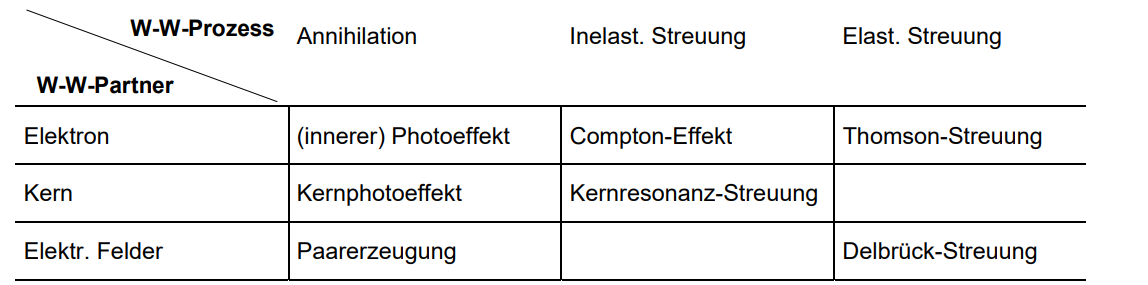
\includegraphics[height=40mm]{bilder/Ab1.png}
    \caption{Die verschiedenen Wechselwirkungen von $\gamma$-Strahlung mit Materie \cite{a1}. \label{Abbildung1} }
\end{figure}

\begin{flushleft}
      Die wesentlichen Prozesse die eintreten sind der Photoeffekt, der Compton-Effekt und die Paarbildung. 
      Der Photoeffekt tritt bei Wechselwirkung des $\gamma$-Quants mit einem Hüllenelektron auf. 
      Das Photon wird dabei vernichtet und die Energie vollständig an das Elektron abgegeben, nach überwinden der Bindungsenergie, was dazu führt, dass das Elektron aus seiner Bindung entfernt wird.
      Beim Compton-Effekt wird das Photon, im Gegensatz zum Photoeffekt, nicht vernichtet, sondern gibt ein teil seiner Energie an das Hüllenelektron, beim aneinander stoßen, ab.
      Beide werden durch den Stoß von ihrer Ursprünglichen Bahn abgelenkt.
      Der Wirkungsquerschnitt $\sigma_{\text{com}}$, von Klein und Nishina aufgestellt, wird berechnet durch
\end{flushleft}

\begin{equation}
    \sigma_{\text{com}} = 2\,\pi\,\text{r}_{\text{e}}^{2} \left(  \frac{1 + \epsilon}{\epsilon^{2}} \left[ \frac{2(1+\epsilon)}{1+2\epsilon} - \frac{1}{\epsilon}\,\ln(1+2\epsilon) \right]  \frac{1}{2\epsilon}\,\ln(1+2\epsilon)  -\frac{1+3\epsilon}{(1+2\epsilon)^{2}}        \right) \,,\label{5}
\end{equation}

\begin{flushleft}
    $\text{r}_{\text{e}}$ steht dabei für den klassischen Elektronenradius, welcher $\text{r}_{\text{e}} = 2,82 \cdot 10^{-15}\,\unit{\meter}$ beträgt.
    Das $\epsilon$ steht hierbei für das Verhältnis der Quantenenergie zu Ruheenergie des Elektrons, $\epsilon = \frac{\text{E}_{\gamma}}{\text{m}_{0} \text{c}^2}$.
    Bei kleinen Energien gilt für den Wirkungsquerschnitt
\end{flushleft}

\begin{equation}
    \sigma_{\text{Th}} = \frac{8}{3}\,\pi\,\text{r}_{e}^2\,,  \label{6}
\end{equation}

\begin{flushleft}
    welcher auch als Thomsonscher Wirkungsquerschnitt bezeichnet wird, da bei kleinen Energien das $\sigma_{\text{com}}$ energieunabhängig wird.
    Der Absorptionskoeffizient, der durch den Compton-Effekt bedingt ist, wird berechnet durch.
\end{flushleft}

\begin{equation}
    \mu_{\text{com}} = \frac{\text{z}\,\text{N}_{\text{L}}\,\rho}{\text{M}}\,\sigma_{\text{com}}\,. \label{7}
\end{equation}

\begin{flushleft}
    Die Paarbildung tritt auf, wenn die Energie des $\gamma$-Quants mindestens doppelt so hoch ist, wie die Ruhemasse eines Elektrons.
    Bei dieser Wechselwirkung entstehen ein Elektron und ein Positron.
    In Abbildung \ref{Abbildung2} wird der Verlauf, anhand von Germanium, des Absorptionskoeffizient in Abhängigkeit der Energie verbildlicht. 
\end{flushleft}

\begin{figure}[H]
    \centering
    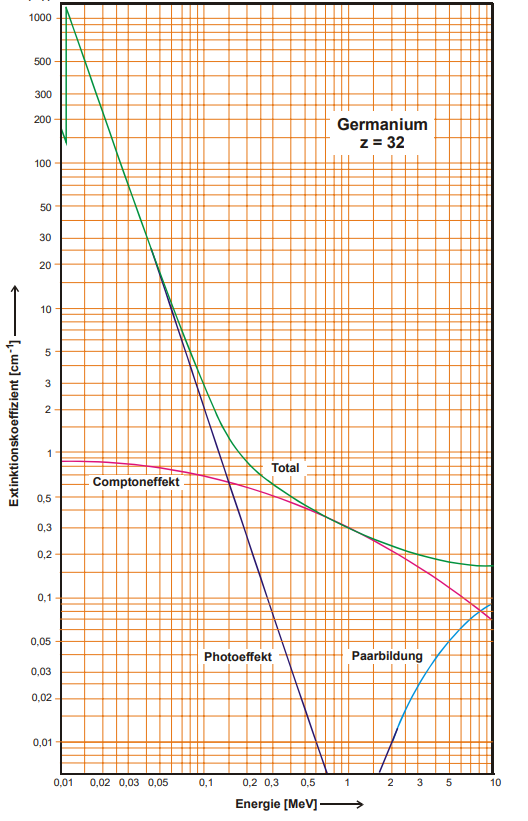
\includegraphics[height=135mm]{bilder/Ab2.png}
    \caption{Energieabhängigkeit des Absorptionskoeffizienten µ für Germanium getrennt nach den verschiedenen Wechselwirkungsmechanismen sowie Totaleffekt \cite{a1}. \label{Abbildung2} }
\end{figure}

\subsection{\textbeta -Strahlung}

\begin{align}
    \intertext{$\beta$-Strahlung besteht aus Elektronen, welche eine hohe Geschwindigkeit besitzen.
    Diese enstehen durch den Zerfall im Atomkern}
    \text{n} \to  \text{p} + \beta^{-} + \overline{\text{v}}_{\text{e}}\,.  \label{8}
    \intertext{$\text{v}_{\text{e}}$ entspricht einem Antineutron und $\overline{\text{v}}_{\text{e}}$ einem Antineutrino, welches neben dem emittierten Elektron als weiteres Elementarteilchen emittiert wird.
    Die bei der Emission frei werdende Energie verteilt sich auf das Elektron und das Neutrino, wobei die Erhaltung dieser Energie durch die gleichzeitige Emission des Neutrinos gesichert wird. 
    Beim Durchlaufen von $\beta$-Strahlung durch Materie treten drei Prozesse auf, bevor das Elektron vollständig absorbiert wird oder austreten kann. } \notag
\end{align}

\begin{flushleft}
    Eine der drei Streuungsprozesse ist die \textbf{Rutherford-Streuung}.
    Diese ist eine elastische Streuung, bei der an den Kernen eine geringe Energieabnahme und starke Richtungsänderung der Teilchenbahn auftritt.\\
    Ein weiterer Streuungsprozess ist die \textbf{inelastische Streuung an Atomkernen}.
    Bei dieser Streuung wird das $\beta$-Teilchen im Coulomb-Feld des Atomkerns beschleunigt, sodass nach quantenmechanischer Theorie energiereiche Photonenergie abgegeben wird.
    Der letzte Streuungsprozess ist die \textbf{inelastische Streuung an den Elektronen}, bei der nur ein Bruchteil der $\beta$-Strahlungsenergie verbraucht wird.
    Dabei ist es in der Lage eine Vielzahl von Ionisations- und Anregungsprozesse hintereinander auszuführen.
\end{flushleft}

\begin{flushleft}
    Wie bei der $\gamma$-Strahlung erfährt die $\beta$-Strahlung ebenfalls einen exponentiellen Abfall.
    Liegt die Dicke nah an der maximal Reichweite, so gilt der Verlauf nicht mehr.
    Nach der maximalen Reichweite $\text{R}_{\text{max}}$ \\
    Bei Logarithmierung beider Strahlungsintensitäten kann, wie in Abbildung \ref{Abbildung3} zu sehen, die maximale Reichweite bestimmt werden.
    Die Reichweite R wird berechnet durch
\end{flushleft}

\begin{equation}
     \text{R} = \rho\,\text{D}\,. \label{9}
\end{equation}

\begin{flushleft}
    Da die maximale Reichweite der $\beta$-Teilchen größtenteils durch die energiereichsten Elektronen bestimmt ist, folgt die maximal freiwerdende Gesamtenergie durch
\end{flushleft}

\begin{equation}
    \text{E}_{\text{max}} = 1,92 \cdot \sqrt{\text{R}_{\text{max}}^2 + 0,22\,\text{R}_{\text{max}}}\,. \label{10}
\end{equation}

\begin{figure}[H]
    \centering
    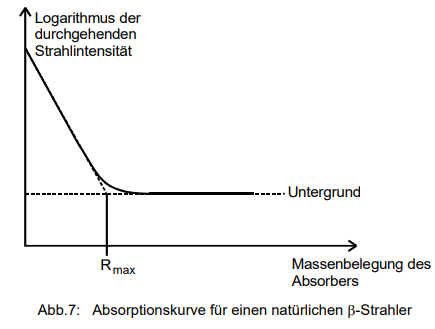
\includegraphics[height=60mm]{bilder/Ab3.png}
    \caption{Absorptionskurve für einen natürlichen β-Strahler \cite{a1}. \label{Abbildung3} }
\end{figure}